\subsubsection{Mô hình cho tập dữ liệu chỉ bao gồm các quan sát có cột "emailtotal" chỉ là giá trị null}


\begin{enumerate}[label=(\alph*)]
    \item Đầu vào mô hình là vector thu được từ phân tích thành phần chính sử dụng thuật toán PCA
    
    Ta có bảng kết quả huấn luyện mô hình:

    \begin{python}
                    precision    recall  f1-score   support

   Keeping house       0.00      0.00      0.00        55
           Other       0.00      0.00      0.00        23
         Retired       0.39      0.42      0.41       113
          School       0.00      0.00      0.00        13
Temp not working       0.00      0.00      0.00         8
Unempl, laid off       0.00      0.00      0.00        19
Working fulltime       0.48      0.87      0.62       198
Working parttime       0.00      0.00      0.00        55

        accuracy                           0.46       484
       macro avg       0.11      0.16      0.13       484
    weighted avg       0.29      0.46      0.35       484
    \end{python}

    và ma trận nhầm lẫn:

    \begin{figure}[H]
        \centering
        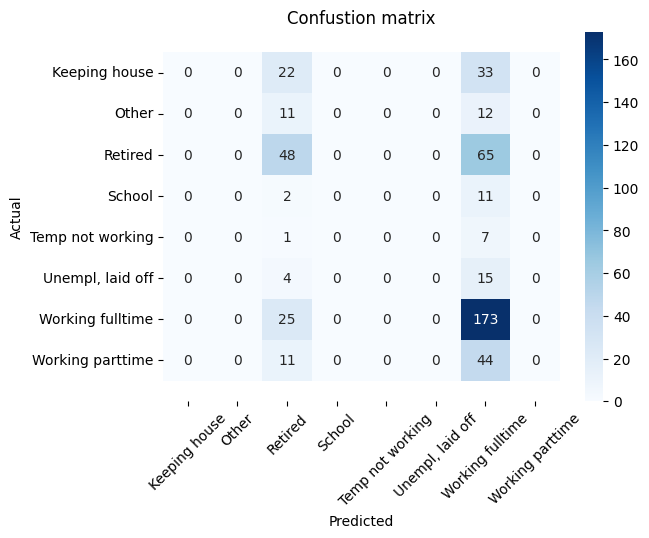
\includegraphics[width=0.6\textwidth]{figures/Thanh/Models/Logistic/With_null_models_confusion_matrix_Logistic_PCA_features.png}
        \caption{Ma trận nhầm lẫn của mô hình Multinomial Logistic Regression khi vector đầu vào được phân tích thành phần chính}
        \label{fig:With_null_models_confusion_matrix_Logistic_PCA_features}
    \end{figure}

    Ta nhận thấy kết quả phân loại không tốt, trừ nhóm làm việc toàn thời gian có độ hồi tưởng là 0.62 và nhóm đã nghỉ hưu có độ hồi tưởng là 0.41 và độ chính xác là 0.53 thì tất cả độ chính xác và độ hồi tưởng của các lớp khác đều bằng 0.
    Nhìn vào ma trận nhầm lẫn ở hình \ref{fig:With_null_models_confusion_matrix_Logistic_PCA_features} ta nhận thấy mô hình dự đoán tất cả các quan sát vào lớp làm việc toàn thời gian.
    Lý do là vì từ phần phân tích dữ liệu, ta thấy phân phối của các thành phần chính tương ứng với các nhóm trong cột wrkstat gần như cùng hình dạng, trộn lẫn vào nhau.
    Mô hình sẽ khó phân biệt được quan sát nào thuộc lớp nào.
    Trong quá trình học, mô hình biết số quan sát thuộc lớp làm việc toàn thời gian và lớp đã nghỉ hưu có số lượng nhiều nhất.
    Từ phần dữ liệu, khi vẽ boxplot của thành phần chính tương ứng với các lớp trong cột wrkstat thì cũng có một chút sự khác biệt giữa hai lớp làm việc toàn thời gian và lớp đã nghỉ hưu (\ref{fig:With_null_boxplot_PCA_features_vs_wrkstat_labels}) và hai lớp này có số quan sát lớn nhất.

    Ta sẽ phân tích ngược trở lại trọng số của các tham số tương ứng với các đặc trưng của vector ban đầu từ các tham số ứng với các đặc trưng của các thành phần chính:

    \begin{figure}[H]
        \centering
        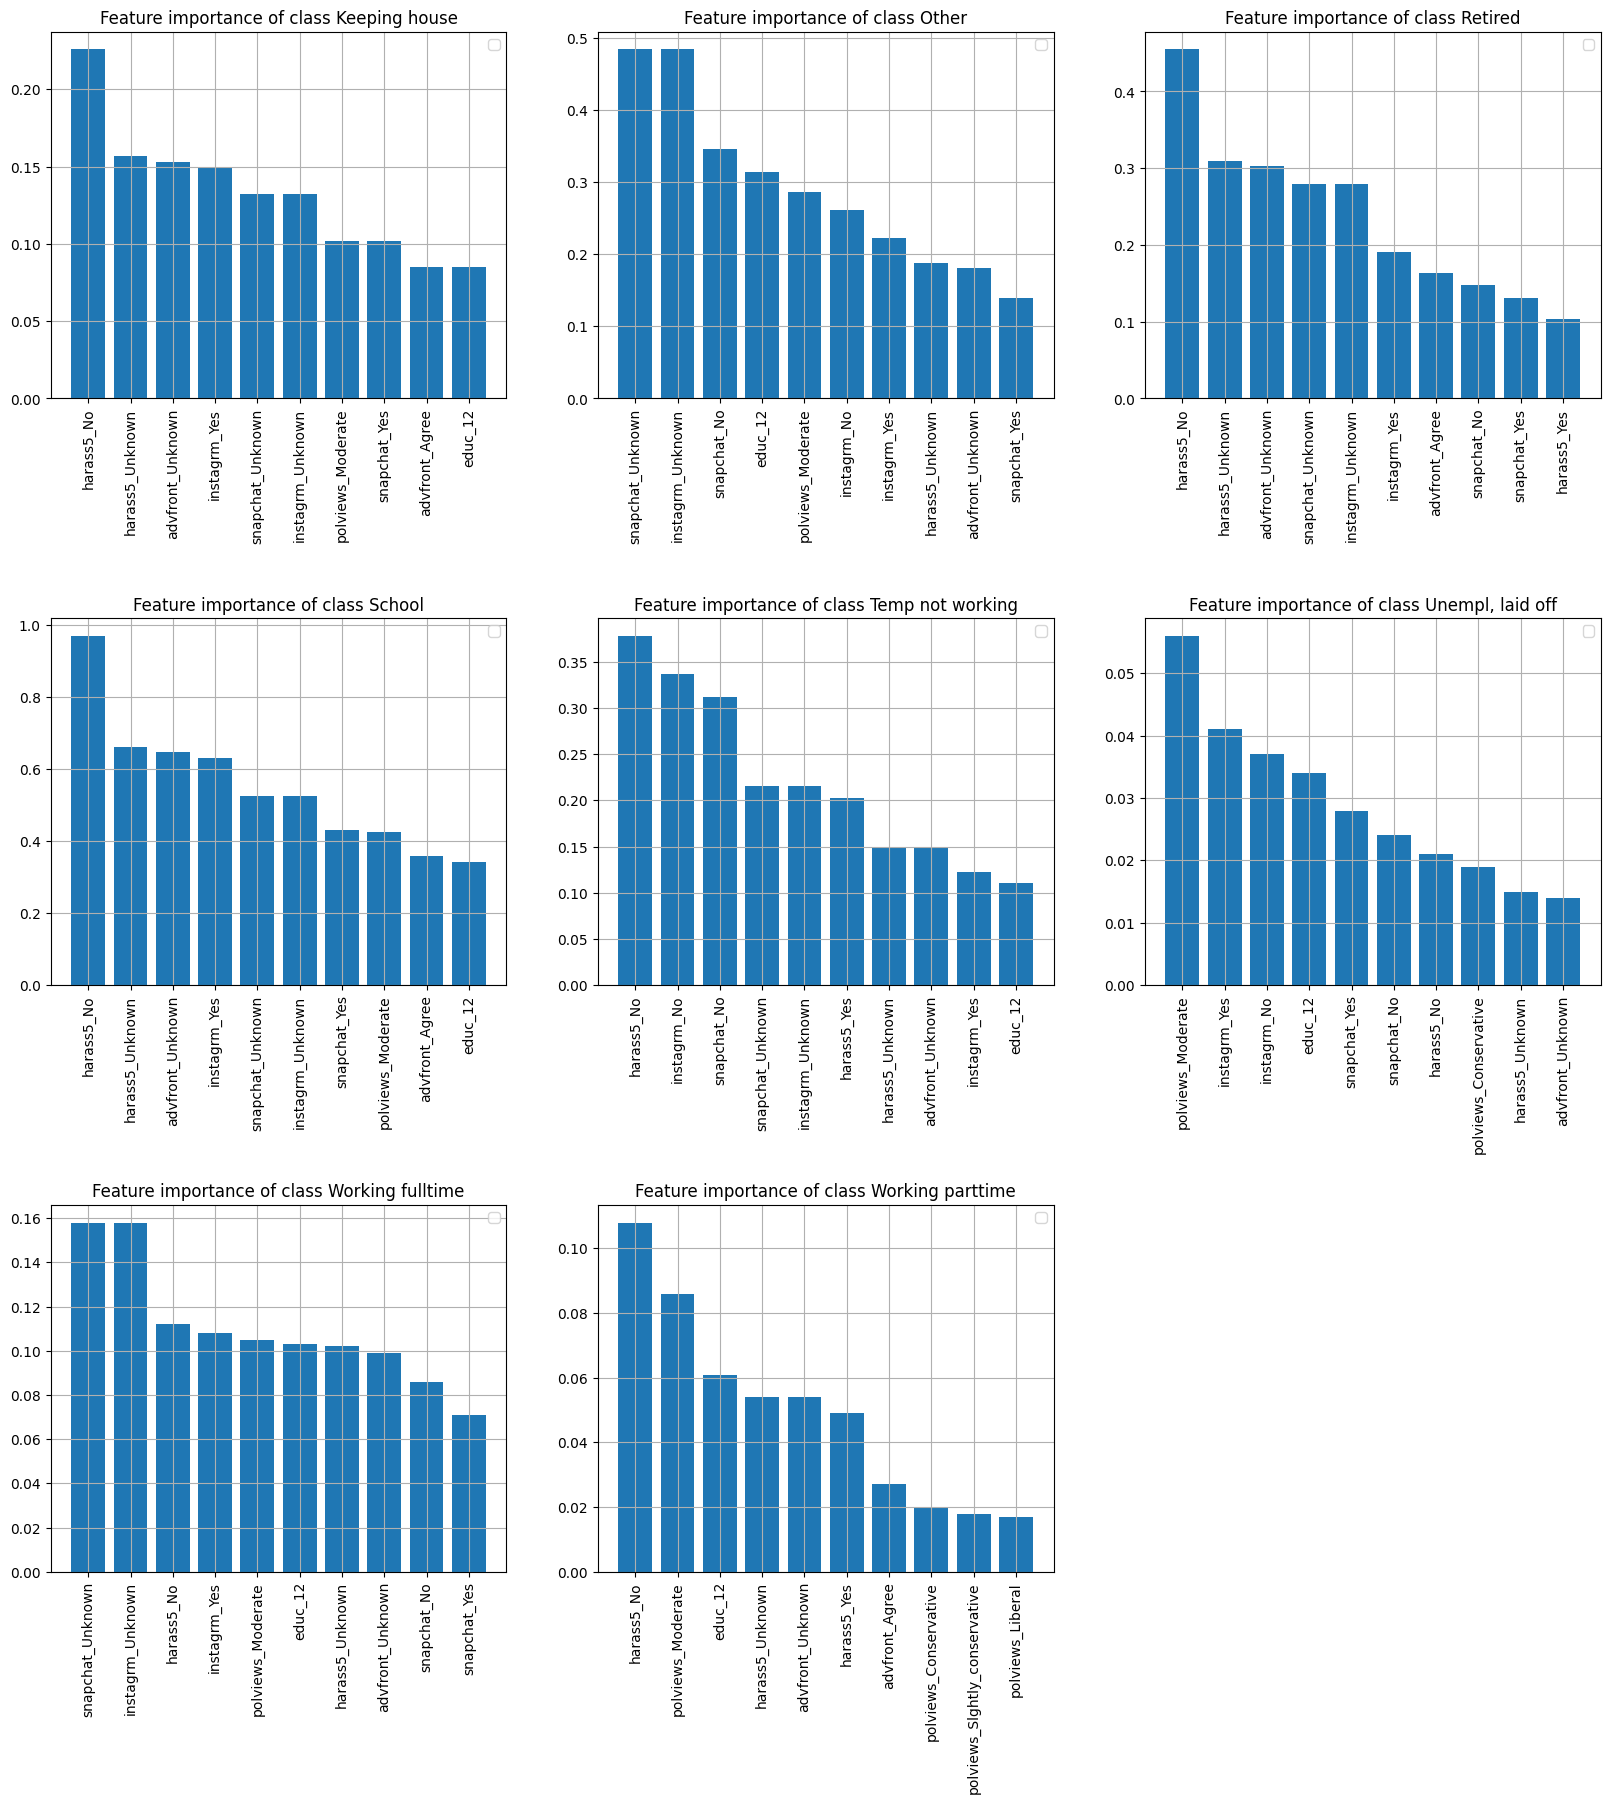
\includegraphics[width=0.6\textwidth]{figures/Thanh/Models/Logistic/With_null_models_Feature_Importance_Logistic_PCA_features.png}
        \caption{Biểu đồ cột sắp xếp độ lớn giảm dần (trị tuyệt đối) tham số của các đặc trưng ứng với từng nhãn}
        \label{fig:With_null_models_Feature_Importance_Logistic_PCA_features}
    \end{figure}

    Ta có biểu đồ cột sắp xếp độ lớn giảm dần (trị tuyệt đối) tham số của các đặc trưng ứng với từng nhãn giả thể hiện ở hình \ref{fig:With_null_models_Feature_Importance_Logistic_PCA_features}.
    Ta nhận thấy các cột có trọng số lớn và ảnh hưởng nhiều tới các các nhãn đầu ra là harass5\_No, snapchat\_Unknown và instagrm\_Unknown.
    Cả ba đặc trưng trên đều có tần suất xuất hiện lớn trong tập dữ liệu.

    \begin{figure}[H]
        \centering
        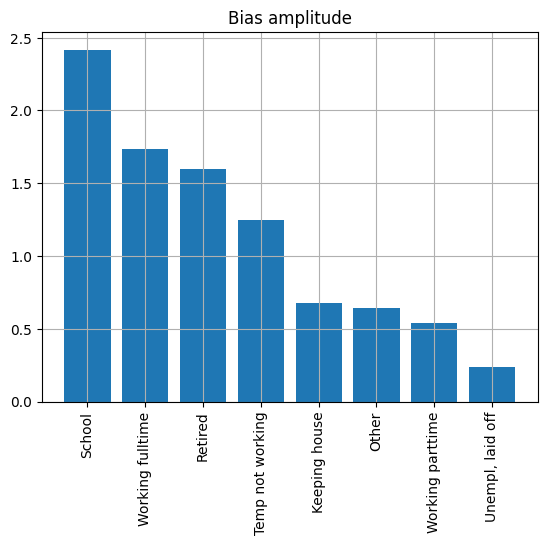
\includegraphics[width=0.6\textwidth]{figures/Thanh/Models/Logistic/With_null_models_Bias_Importance_Logistic_PCA_features.png}
        \caption{Biểu đồ cột thể hiện độ lớn của các bias tương ứng với từng nhãn}
        \label{fig:With_null_models_Bias_Importance_Logistic_PCA_features.png}
    \end{figure}

    Hình \ref{fig:With_null_models_Bias_Importance_Logistic_PCA_features.png} thể hiện độ lớn của các bias tương ứng với từng nhãn.
    Tuy nhiên độ lớn của bias tương ứng với hai nhãn làm việc thời gian và nhãn đã nghỉ hưu cao xếp sau nhãn School (đang đi học).
    
    \item Vector đầu vào là vector gốc ban đầu

    Ta có bảng kết quả huấn luyện mô hình:

    \begin{python}
                    precision    recall  f1-score   support

   Keeping house       0.12      0.04      0.06        55
           Other       0.00      0.00      0.00        23
         Retired       0.39      0.51      0.45       113
          School       0.00      0.00      0.00        13
Temp not working       0.00      0.00      0.00         8
Unempl, laid off       0.00      0.00      0.00        19
Working fulltime       0.51      0.82      0.63       198
Working parttime       0.00      0.00      0.00        55

        accuracy                           0.46       484
       macro avg       0.13      0.17      0.14       484
    weighted avg       0.32      0.46      0.37       484
    \end{python}

    và ma trận nhầm lẫn:

    \begin{figure}[H]
        \centering
        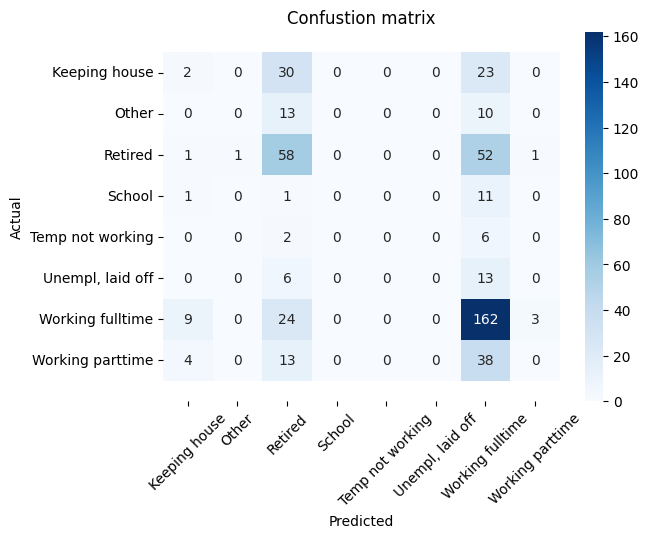
\includegraphics[width=0.6\textwidth]{figures/Thanh/Models/Logistic/With_null_models_confusion_matrix_Logistic_original_features.png}
        \caption{Ma trận nhầm lẫn của mô hình Multinomial Logistic Regression khi vector đầu vào là vector gốc ban đầu}
        \label{fig:With_null_models_confusion_matrix_Logistic_original_features}
    \end{figure}

    Ta nhận thấy kết quả gần như không khác nhiều so với trường hợp mô hình đầu vào là vector đã được phân tích thành phần chính sử dụng thuật toán PCA.
    Độ chính xác và độ hồi tưởng của lớp làm việc toàn thời gian cao hơn chút và độ hồi tưởng của lớp đã nghỉ hưu cao hơn một chút so với trường hợp trên.
    Lý do là vì khi sử dụng vector gốc ban đầu, mô hình có nhiều thông tin hơn để phân loại các lớp.
    Tuy vậy, phân phối dữ liệu vẫn chưa đủ tách biệt giữa các lớp khác nhau chưa đủ để mô hình có thể học được cách phân loại tốt các lớp trong cột wrkstat.

    Ta sẽ phân tích ngược trở lại trọng số của các tham số tương ứng với các đặc trưng của vector ban đầu từ các tham số ứng với các đặc trưng:

    \begin{figure}[H]
        \centering
        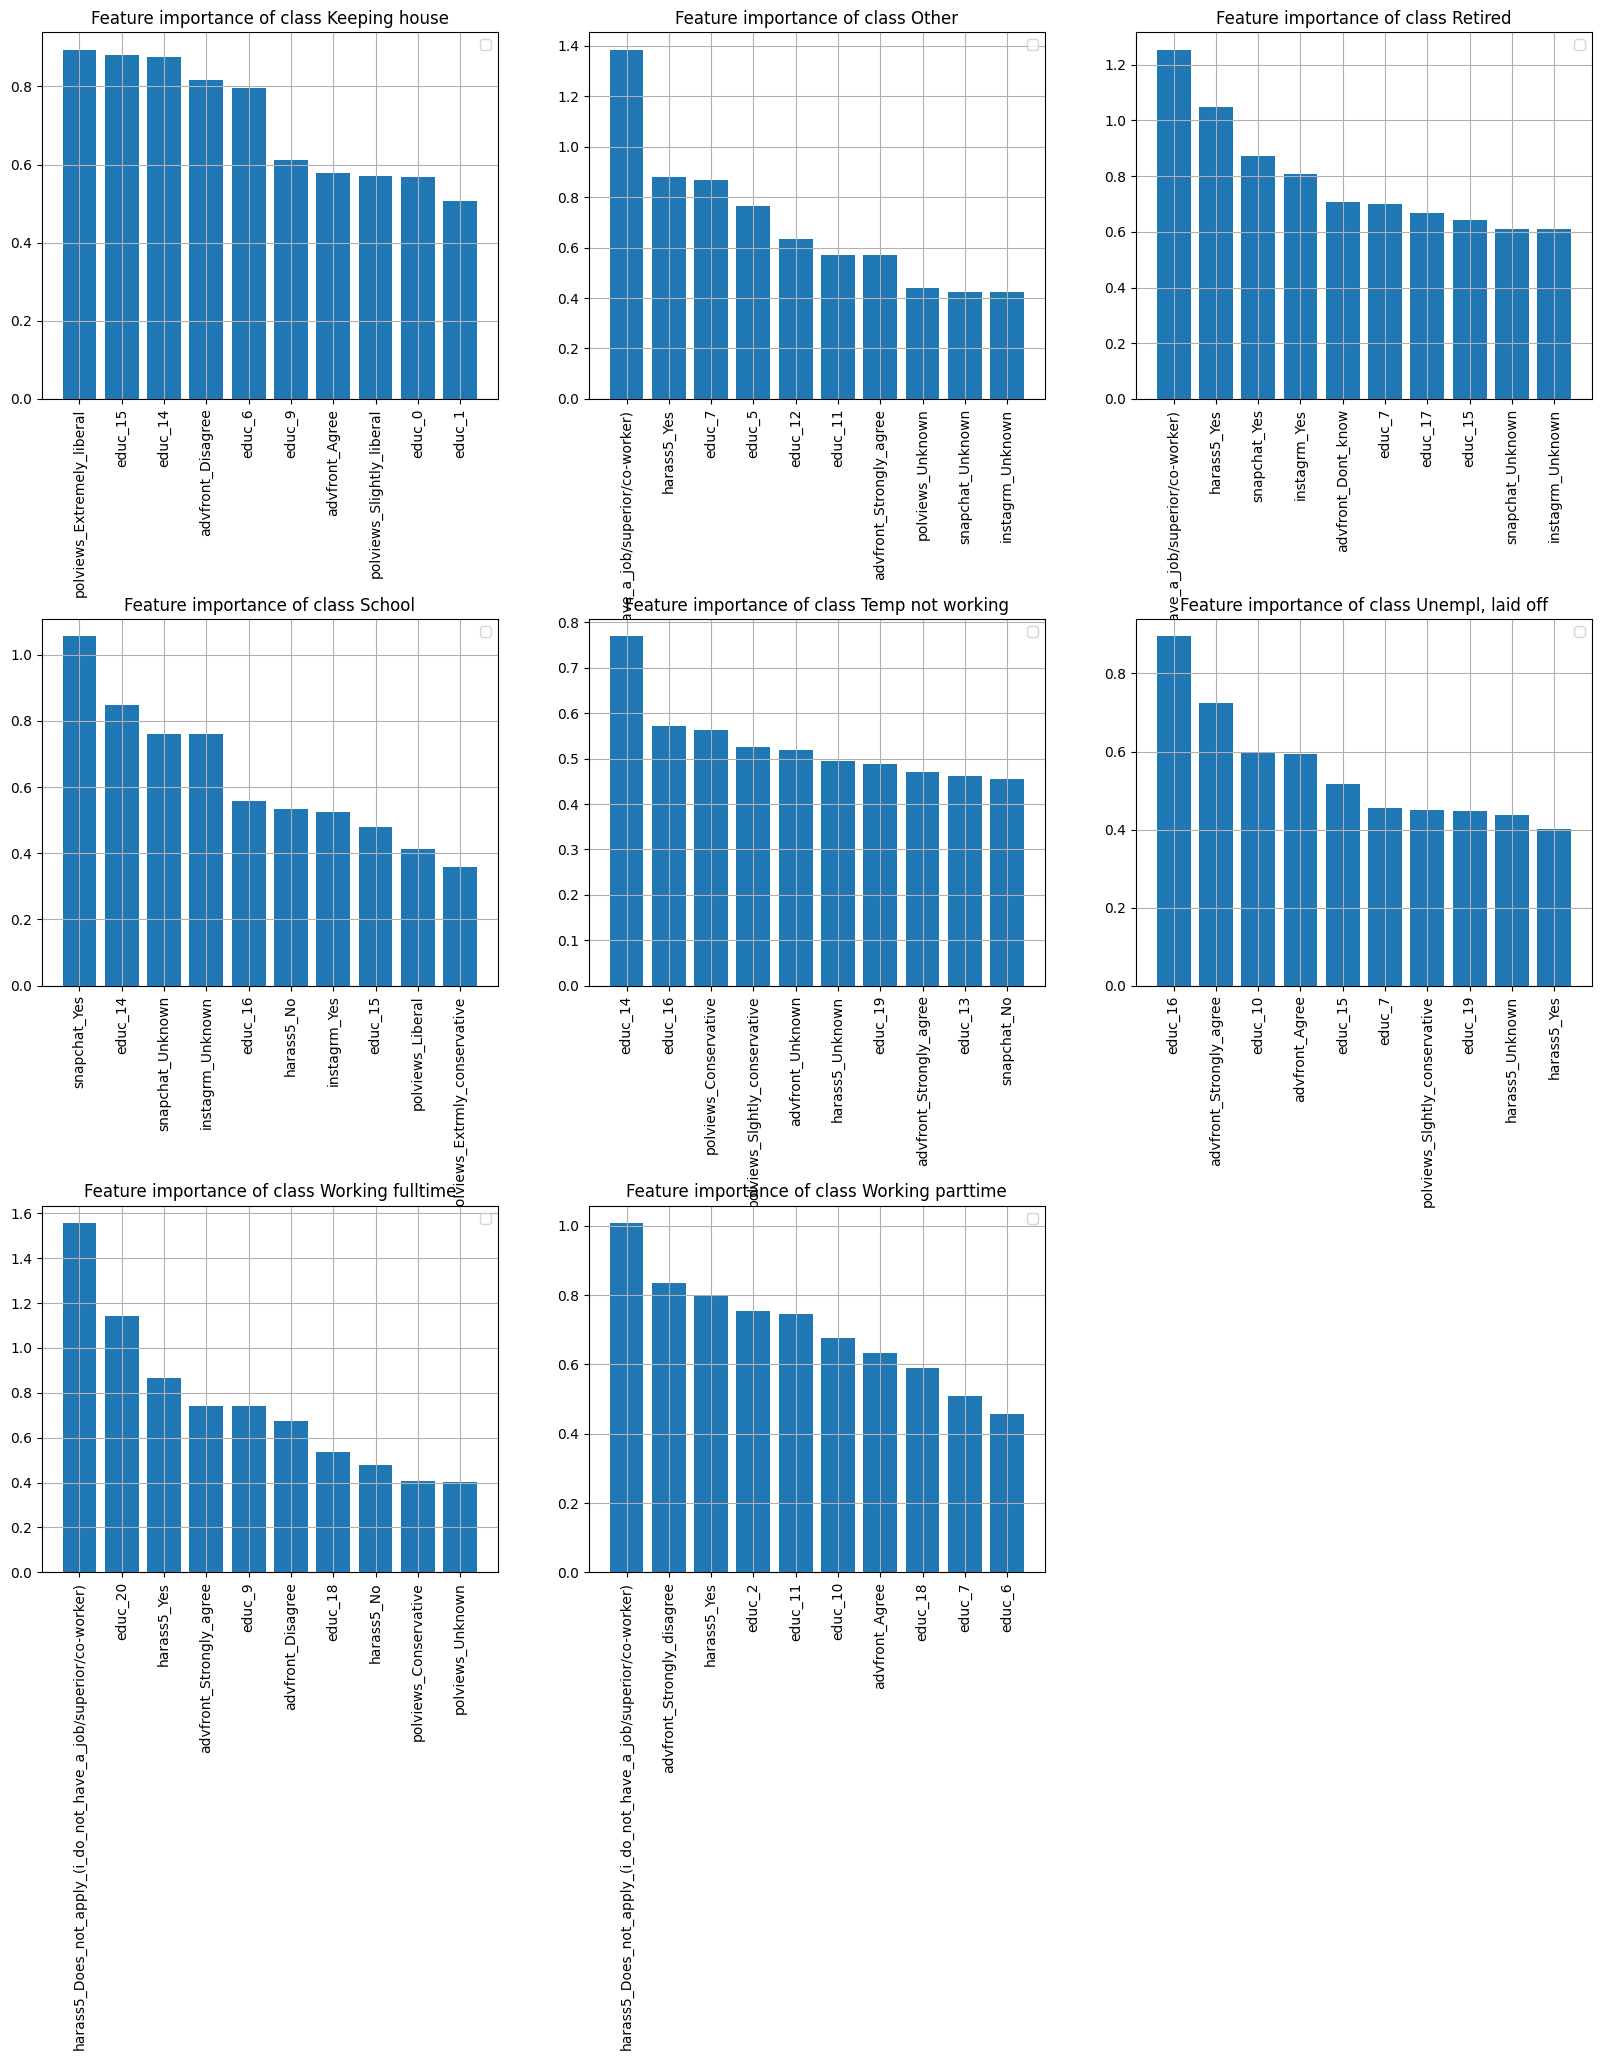
\includegraphics[width=0.6\textwidth]{figures/Thanh/Models/Logistic/With_null_models_Feature_Importance_Logistic_original_features.png}
        \caption{Biểu đồ cột sắp xếp độ lớn giảm dần (trị tuyệt đối) tham số của các đặc trưng ứng với từng nhãn giả (mô hình với vector đầu vào là vector gốc ban đầu)}
        \label{fig:With_null_models_Feature_Importance_Logistic_original_features}
    \end{figure}

    Ta có biểu đồ cột sắp xếp độ lớn giảm dần (trị tuyệt đối) tham số của các đặc trưng ứng với từng nhãn giả thể hiện ở hình \ref{fig:With_null_models_Feature_Importance_Logistic_original_features}.
    Ta nhận thấy các đặc trưng có trọng số lớn tương ứng với từng lớp là educ\_14, educ\_16, snapchat\_Yes, harass5\_Does\_not\_apply đa số là các đặc trưng ít xuất hiện trong tập dữ liệu.

    \begin{figure}[H]
        \centering
        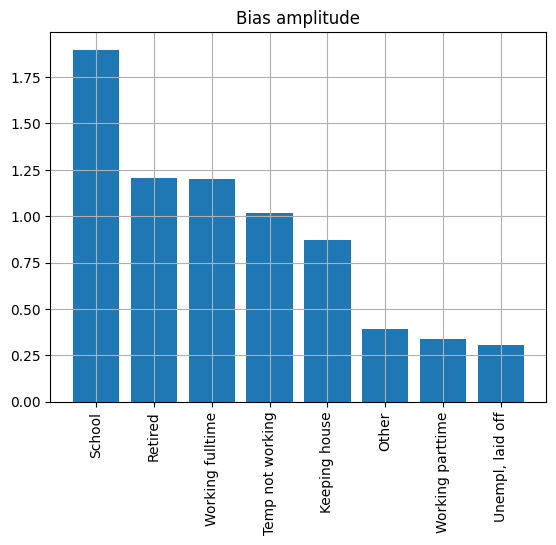
\includegraphics[width=0.6\textwidth]{figures/Thanh/Models/Logistic/With_null_models_Bias_Importance_Logistic_original_features.png}
        \caption{Biểu đồ cột thể hiện độ lớn của các bias tương ứng với từng nhãn giả (mô hình với vector đầu vào là vector gốc ban đầu)}
        \label{fig:With_null_models_Bias_Importance_Logistic_original_features.png}
    \end{figure}

    Hình \ref{fig:With_null_models_Bias_Importance_Logistic_original_features.png} thể hiện độ lớn của các bias tương ứng với từng nhãn.
    Tuy nhiên độ lớn của bias tương ứng với hai nhãn làm việc thời gian và nhãn đã nghỉ hưu cao xếp sau nhãn School (đang đi học).
\end{enumerate}